\documentclass[a4paper,oneside,article,11pt]{memoir}
\usepackage[english]{babel}
\usepackage[utf8]{inputenc}
\usepackage{amsmath,amssymb,amsthm}

% This font looks so good.
\usepackage[sc]{mathpazo}

% Typesetting pseudo-code
\usepackage{algorithm}
\usepackage{algorithmic}
\usepackage{multirow}
% Code comments like [CLRS]
\renewcommand{\algorithmiccomment}[1]{\makebox[5cm][l]{$\triangleright$ \textit{#1}}}
\usepackage{framed,graphicx,xcolor}
\usepackage[font={small,it}]{caption}
\usepackage{listings}
\usepackage{units}

% Relative references
\usepackage{varioref}

\usepackage{hyperref}

\bibliographystyle{plain}

\title{Advanced Data Structures \\ Project 2 - van Emde Boas Trees}
\author{Peter Gabrielsen 20114179 \\
Christoffer Hansen 20114637}
\newcounter{qcounter}
\begin{document}

\begin{titlingpage}
\clearpage

\maketitle
\thispagestyle{empty}

\begin{abstract}
missing
\\
\\
\\
The code can be found at: \\\url{Insert link to code here!}.
\end{abstract}
\end{titlingpage}

\pagebreak

\tableofcontents

\pagebreak

\chapter{Introduction}


\chapter{Implementation}
\label{cpt:implementation}


\subsection{van Emde Boas tree}
The van Emde Boas tree was implemented as described in Introduction to Algorithms~\cite{clrs}. It is a non space-reduced tree and as such it will take time proportional to allocating the full universe of the tree in memory, to construct such a tree. However the tree will not grow in memory after allocation. A way to mitigate this, and thereby make the tree space-reduced would be to, instead of storing the complete structure, we should only store the substructures that actually contain elements. This could have been implemented by using hash maps instead of arrays.

\subsection{Red-Black tree}
The Red-Black tree was implemented as described in Introduction to Algorithms~\cite{clrs}

\chapter{Experimental setup}
\label{chtp:experiment_setup}
%TODO write something about the machine which ran the experiments and something about how we measure the different things. Maybe copy all this from the AE report?

The experiments were performed on a machine with a Intel i5-3210M @ 2.5GHz (Ivy Bridge) with 128K bytes of L1 cache, 512K bytes of L2 and 3072K bytes of L3 cache. The machine had 4.2GB ram and ran Ubuntu 14.04 with kernel version 3.16.0-50.

The running time was measured using the built in \texttt{high\_resolution\_clock} in the \texttt{chrono} library. This measures the wall clock. It is the clock in \texttt{c++} with the highest precision, i.e. the shortest tick period.

The code is compiled with \texttt{g++ 4.8.4} with the \texttt{c++11} standard enabled and no optimization level.

The elements in our data structures were 32 bit integers. Random elements were generated uniformly in the 32 bit integer range using the Mersenne Twister 19937 from the \texttt{random} library.

CPU measurements were collected using \texttt{PAPI 5.3.0.0}

We used \texttt{perf} to measure page faults.

\chapter{Priority queue experiments}
\label{heap_experiments}
In this section we will design and perform experiments where we compare the van Emde Boas tree based priority queue with more standard priority queue implementations, namely the Fibonacci heap and binary heap. We will for each priority queue operation describe the experiments, present the results of said experiments and discuss those in detail.

\section{\texttt{FindMin}}
Finding the minimum in all three priority queues are constant time operations. They all just involve returning a stored element or dereferencing a pointer. We therefore expect to see all three queues perform similar and constant in the size of the input. In this experiment we do not measure running time since this is a constant time operation. Instead we measure the number of cycles and branch operations performed when calling find minimum in the respective queues. The experiments are repeated 10 times and averaged. The results are depicted in figure~\ref{fig:findmin_br} and~\ref{fig:findmin_cyc}.

\begin{figure}[H]
\centering
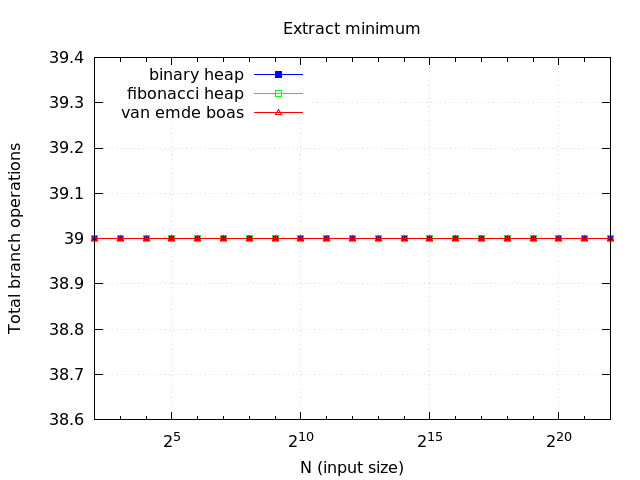
\includegraphics[scale=0.5]{../res2/findmin/extract_min_branch.png}
\caption{Number of branch operations for finding the minimum element}
\label{fig:findmin_br}
\end{figure}

\begin{figure}[H]
\centering
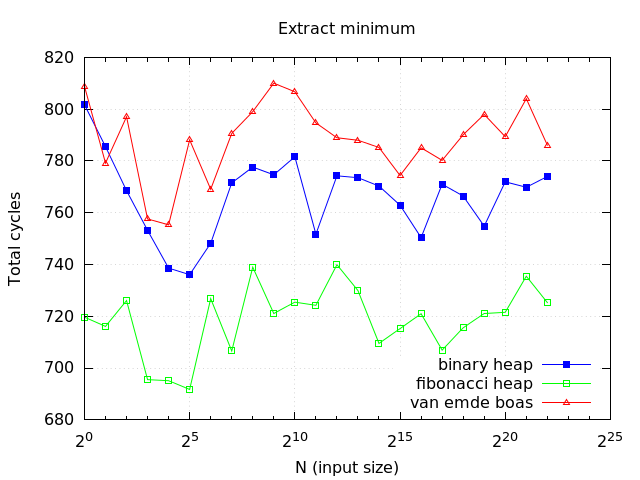
\includegraphics[scale=0.5]{../res2/findmin/extract_min_cycles.png}
\caption{Number of cycles for finding the minimum element}
\label{fig:findmin_cyc}
\end{figure}

The results clearly depict that finding the minimum does not depend on the input size and we conclude that the theoretical bound of $\mathcal{O}(1)$ also matches the experimental found results.

\section{\texttt{Insert}}


\section{\texttt{DeleteMin}}

\section{\texttt{DecreaseKey}}


\section{Conclusion}


\chapter{Red-Black tree \& van Emde Boas}


\chapter{Conclusion}


\bibliography{references}

\end{document}


